\documentclass[a4paper, notitlepage, 12pt]{scrartcl}
\author{Lukas Rost \\ \small{Teilnahme-ID: 44137}}
\title{Aufgabe 1 \\ \glqq Die Kunst der Fuge\grqq  - Dokumentation}
\subtitle{36. Bundeswettbewerb Informatik 2017/18 - 2. Runde \\~\\}
\date{9. April 2018}
\usepackage[ngerman]{babel}
\usepackage[utf8]{inputenc}
\usepackage{graphicx}
\usepackage{wrapfig}
\usepackage{color}
\usepackage[dvipsnames]{xcolor}
\usepackage{hyperref}
\usepackage[top=2.5cm, bottom=1.5cm, left=2.5cm, right=2.5cm]{geometry}
\usepackage{fancyvrb}
\usepackage{caption}
\usepackage{mathtools}
\usepackage{amssymb}
\usepackage{fancyhdr}
\usepackage{lastpage}
\usepackage{multicol}
\usepackage{pgfplots}
\pgfplotsset{compat=1.15}
\usepackage{tikz}

\DeclarePairedDelimiter\floor{\lfloor}{\rfloor}

\usepackage{minted}
\fvset{breaklines=true}

\pagestyle{fancy}
\lhead{Lukas Rost, Teilnahme-ID: 44137}
\rhead{Aufgabe 1, Seite \thepage ~von \pageref{LastPage}}
\cfoot{ }

\newenvironment{longlisting}{\captionsetup{type=listing}}{}

\newmintedfile{java}{frame=single,linenos,samepage=false,firstnumber=1,rulecolor=\color{Gray},autogobble,breakafter=.u,fontsize=\small}

\begin{document}
\renewcommand{\contentsname}{\centerline{Inhaltsverzeichnis}}
 \maketitle
 \tableofcontents
 \thispagestyle{empty}
 \newpage
 \setcounter{page}{1}
 
 \section{Lösungsidee}
 \subsection{Mögliche Maximalhöhe der Mauer}
 Da in der Aufgabe explizit nach der Höhe der Mauer für verschiedene $n$ gefragt ist, lohnt es sich, diese zunächst einmal mathematisch zu berechnen. Damit lässt sich der Suchraum effektiv eingrenzen, da ab dieser Maximalhöhe die Forderungen der Aufgabenstellung nicht mehr erfüllt werden können. Pro Reihe der Mauer gibt es $n-1$ verschiedene Fugen. Diese Zahl ergibt sich daraus, dass hinter jedem Klötzchen genau eine Fuge folgt. Nur beim letzten Klötzchen der Reihe zählt diese Position nicht, da sich dahinter kein weiteres Klötzchen befindet. \\ \\
Fugen sind also per Definition nur die Stellen zwischen den Klötzchen, da die Position 0 sowie die Position $\frac{n \cdot (n+1) }{2}$ am Ende der Reihe in jeder Reihe belegt werden. Nun interessiert noch die Zahl der insgesamt belegbaren Fugenpositionen. Dies sind alle Positionen von 1 bis zur Länge der Mauer minus 1\footnote{Hier ist jeweils der Abstand zum linken Rand der Mauer gemeint.}, da, wie bereits erwähnt, die Position am Ende nicht als Fuge zählt. Die Länge der Mauer ist die Summe aller natürlichen Zahlen bis $n$, also nach der Gaußschen Summenformel $\frac{n \cdot (n+1) }{2}$. \\ \\
Teilt man nun die Anzahl der insgesamt verfügbaren Fugenpositionen durch die Anzahl der Fugen pro Reihe, erhält man die mögliche Anzahl an Reihen, also die Höhe. 
\begin{equation}
H(n) = \frac{\frac{n \cdot (n+1) }{2} - 1}{n - 1} = \frac{(n + 2) \cdot (n - 1)}{2 \cdot (n - 1)} = \floor{\frac{n + 2}{2}}
\end{equation}
Die Abrundungsfunktion ist an dieser Stelle nötig, da sonst für ungerade $n$ das Resultat keine natürliche Zahl ist. Halbe Reihen jedoch ergeben wenig Sinn. Die angegebene Funktion $H(n)$ ist für alle natürlichen Zahlen $ n \geq 2$ definiert. \\ \\
Der Fall $ n = 1$ ist damit nicht berechenbar, da in der Originalgleichung durch 0 geteilt würde. Dieser muss auch ausgeschlossen werden, da es dabei keine Fugen im Sinne von Stellen zwischen den Klötzen gibt. Somit ist nicht eindeutig definiert, ob in diesem Fall nur eine Reihe (mit einem Klotz der Länge 1) oder unendlich viele Reihen erlaubt sind. \\ \\
Die obere Schranke (für die Höhe) von $\frac{n + 2}{2}$ wird bei ungeraden $n$ nie erreicht. Das bedeutet, dass in diesem Fall immer Fugenpositionen offen bleiben und nicht belegt werden.
\begin{figure}[H]
	\centering
	\begin{tikzpicture}[scale=.75]
		\draw[very	thick] (0, 0) rectangle (1, 1) (1, 0) rectangle (4, 1) (4, 0) rectangle (6, 1) (6, 0) rectangle (11, 1) (11, 0) rectangle (15, 1) (0, 1) rectangle (2, 2) (2, 1) rectangle (5, 2) (5, 1) rectangle (9, 2) (9, 1) rectangle (14, 2) (14, 1) rectangle (15, 2) (0, 2) rectangle (3, 3) (3, 2) rectangle (7, 3) (7, 2) rectangle (8, 3) (8, 2) rectangle (13, 3) (13, 2) rectangle (15, 3);

		\draw[thick, dashed] (10, -.25) node[above] {} -- (10, 3.25);
		\draw[thick, dashed] (12, -.25) node[above] {} -- (12, 3.25);
	\end{tikzpicture}
	\caption{Offene Fugenpositionen bei ungeraden $n$}
\end{figure}
Die Anzahl der offenen Fugenpositionen($\ell$) für ungerade $n$ ist ebenfalls berechenbar, denn sie ist die Differenz aus der Anzahl aller Fugenpositionen $\frac{n(n+1)}{2} - 1$ und der Anzahl besetzter Fugenpositionen $H \cdot (n-1)$. Damit ergibt sich:
\begin{align*}
	\ell &= \frac{1}{2} \cdot(n-1)
\end{align*}
\begin{figure}[H]
\begin{center}
\begin{tikzpicture}
\begin{axis}[axis lines=middle, xlabel=$n$,
    ylabel={$H(n) = \floor{\frac{n+2}{2}}$}, grid,xmin=0, xmax=20,
    ymin=0, ymax=11,
    xtick={2,4,6,8,10,12,14,16,18,20}]
\foreach \n in {2,3,4,5,6,7,8,9,10,11,13,14,15,17,18,19,20}{
    \addplot [mark=*] coordinates {(\n,{floor((\n/2)+1)})}; 
    }
\foreach \n in {12,16} {
\addplot [mark=*] coordinates {(\n,{floor((\n/2)+1)+1})}; 
    }
\end{axis}
\end{tikzpicture}
\end{center}
\caption{Werte für n = 2,...,20}
\end{figure}
\subsection{Lösungsansatz: Backtracking}
Zunächst kann man davon ausgehen, dass es für jedes beliebige $n$ einer Mauer dieser Maximalhöhe gibt. Nun muss man diese nur noch finden. Der einfachste mögliche Ansatz für dieses Problem wäre es, in jeder Reihe alle Anordnungen der Klötze auszuprobieren. Da es jedoch pro Reihe $n!$ Permutationen der Klötze gibt, ist dieser Brute-Force-Lösungsansatz mit einer Laufzeit in $\mathcal{O}(n!^{\floor{\frac{n + 2}{2}}})$ gänzlich inakzeptabel.
\\ \\
Es wird also ein effizienterer Lösungsalgorithmus für das Problem benötigt. Dabei tritt jedoch das Problem auf, dass es, wie im nächsten Abschnitt besprochen, höchstwahrscheinlich keinen effizienten Lösungsalgorithmus mit polynomialer Laufzeit gibt. Also muss versucht werden, die Brute-Force-Suche effizienter zu gestalten. Ein guter Weg dazu ist rekursives Backtracking.
\\ \\
Zunächst wird für Backtracking ein Lösungsvektor benötigt. In diesem Fall kann das ein zweidimensionales Array sein, dessen erste Dimension die Reihe darstellt und dessen zweite Dimension für jede Reihe von links nach rechts die verwendeten Klötze angibt. Somit stellt dieser anfangs eine leere Mauer dar. \\ \\ Backtracking stellt dabei eine Tiefensuche auf einem impliziten Baum dar. Die Knoten des genannten Baumes stellen dabei die Zustände des Lösungsvektors dar und es existiert eine Kante zwischen Zuständen, die durch Hinzufügen eines Klotzes an das Ende des aktuellen Lösungsvektors auseinander hervorgehen. Die Wurzel des Baumes, an der die Backtracking-Suche begonnen wird, stellt ein leerer Lösungsvektor dar. Die Suche versucht nun, bis in die tiefste Ebene des Baumes vorzudringen, ohne dass Fugenpositionen doppelt belegt werden. Ist die Mauer vollständig gefüllt, so ist der zugehörige Zustands-Knoten eine \emph{Lösung}. Alle Blätter des Baums entstehen entweder durch Pruning ($\times$ im Baum unten) oder sie sind Lösungen ($\checkmark$ im Baum).
\\ \\
Beim Backtracking wird nun also Klotz für Klotz eine Lösung aufgebaut.\footnote{Dadurch sind die Reihen während der Konstruktion nur teilweise gefüllt. In diesem Zustand besitzt jede Reihe eine Länge $\ell$, die der Summe der Längen aller in dieser Reihe enthaltenen Klötze entspricht. Die Reihe endet also vorübergehend an der Fugenposition $\ell$.}  Dabei wird jeweils der längste in dieser Reihe noch nicht verwendete und an dieser Stelle noch nicht ausprobierte Klotz gewählt. Sobald jedoch sicher ist, dass eine solche Teillösung nicht zu einer Gesamtlösung ausgebaut werden kann, kommt das sogenannte Pruning zum Einsatz. Da es sinnlos ist, von einer solchen Teillösung aus weiter in die Tiefe zu gehen, kann man die Wahl des Klotzes auf der aktuellen Stufe rückgängig machen und in die vorherige Stufe zurückwechseln. Dort werden dann alle weiteren aktuellen Wahlmöglichkeiten des Klotzes nach dem gleichen Prinzip durchprobiert.
\begin{figure}[H]
	\centering
	\begin{tikzpicture}[scale=.75, y=8mm]
		\def\checkmark{\tikz\fill[scale=0.4](0, .35) -- (.25, 0) -- (.6, .7) -- (.25, .15) -- cycle;} 
		\tikzstyle{node}=[draw, thick, circle, inner sep=0pt, minimum width=5mm]
		\large
		\node[node] (a) at (0, 6) {};
		\node[node] (b1) at (-4, 4) {};
		\node[node] (b2) at (0, 4) {};
		\node[node] (b3) at (4, 4) {};
		\node[node] (c11) at (-5, 2) {};
		\node[node] (c12) at (-4, 2) {};
		\node[node] (c13) at (-3, 2) {$\times$};
		\node[node] (c22) at (0, 2) {};
		\node[node] (c23) at (1, 2) {$\times$};
		\node[node] (c33) at (4, 2) {$\times$};
		\node[node] (d111) at (-7, 0) {$\times$};
		\node[node] (d112) at (-6, 0) {$\times$};
		\node[node] (d113) at (-5, 0) {$\times$};
		\node[node] (d122) at (-4, 0) {$\times$};
		\node[node] (d221) at (-1, 0) {$\times$};
		\node[node] (d222) at (0, 0) {\checkmark};
		\draw[-{latex}, thick] (a) edge (b1) (a) edge (b2) (a) edge (b3)
		                 (b1) edge (c11) (b1) edge (c12) (b1) edge (c13)
		                 (b2) edge (c22) (b2) edge (c23)
		                 (b3) edge (c33)
		                 (c11) edge (d111) (c11) edge (d112) (c11) edge (d113)
		                 (c12) edge (d122)
		                 (c22) edge (d221) (c22) edge (d222);
	\end{tikzpicture}
	\caption{Beispiel für einen Suchbaum}
\end{figure}
Ein solcher Algorithmus findet in jedem Fall eine maximal hohe Mauer, sofern es eine solche gibt. Es handelt sich hierbei nämlich nur um eine intelligentere Variante der Brute-Force-Suche. Wichtig für die Funktionsfähigkeit dieses Algorithmus ist, dass die Höhe der Mauer durch einen Maximalwert begrenzt ist und wir somit wissen, wann eine vollständige Lösung erreicht ist. Sobald eine solche erreicht ist, kann die Suche auch abgebrochen werden, da nur eine und nicht mehrere Mauern mit maximaler Höhe gesucht sind.
\\ \\
Nun ist es noch wichtig, Pruning-Kriterien so zu definieren, dass möglichst viele nicht ausbaubaren Teillösungen möglichst früh gefunden und solche Teillösungen verworfen werden. Dadurch verringert sich die Größe des betrachteten Teilbaums bis zur vollständigen Lösung.  Bei geeigneten Kriterien lässt sich nämlich die Laufzeit im Vergleich zu Brute Force erheblich verbessern.
\\ \\
\textbf{Pruning-Kriterien}
\\ \\
Es lassen sich zunächst zwei Grundannahmen für die ersten beiden Reihen der Mauer treffen, wodurch diese nicht durch Backtracking ermittelt werden müssen.
\begin{enumerate}
\item Die erste Reihe der Mauer ist im Format $(1,2,3,...,n)$ aufgebaut. Diese Annahme kann gefahrlos getroffen werden, da sich alle anderen Reihen dann danach ausrichten. Dieses Vorgehen führt in der Praxis auch zu richtigen Ergebnissen.
\item Die zweite Reihe der Mauer ist meistens im Format $(2,3,...,n,1)$ aufgebaut. Diese Annahme bestätigt sich, wenn man den Algorithmus unter Verwendung der ersten Annahme implementiert. Lediglich für $n = 6$ und $n = 10$ führt diese Annahme nicht zu gültigen Mauern und darf deshalb dort nicht verwendet werden.
\end{enumerate}
Nun kann man zwei Pruning-Kriterien festlegen.
\begin{enumerate}
\item \textit{Das offensichtliche Kriterium:} Gibt es an einer Stelle keine Möglichkeit mehr, einen in dieser Reihe noch nicht verwendeten Klotz so zur Mauer hinzuzufügen, dass keine Fuge doppelt belegt wird, so ist mit der bisherigen Mauer keine Lösung zu erreichen. Somit kann man hier prunen und auf die nächsthöhere Ebene zurückkehren.
\item \textit{Das erweiterte Kriterium, Teil 1:} Befindet man sich noch nicht in der letzten Reihe und bemerkt, dass zwischen zwei benachbarten noch nicht belegten Fugenpositionen\footnote{Hier zählen auch 0 und $\frac{n \cdot (n+1) }{2}$ als Fugenpositionen im erweiterten Sinne.} der Abstand größer als $n$ ist, so gibt es ebenfalls keine Lösung mit der bisherigen Mauer. Also kann ebenfalls geprunt werden, da kein genügend langer Klotz zur Überwindung dieses Abstands existieren kann.
\item \textit{Das erweiterte Kriterium, Teil 2:} Befindet man sich noch nicht in der letzten Reihe und bemerkt, dass nach der Position, an der die aktuelle Reihe bisher endet, ein ebensolcher Abstand besteht, der größer als der längste in dieser Reihe noch nicht verwendete Klotz ist, ist Pruning ebenfalls möglich. In dieser Reihe müsste dieser Abstand nämlich noch überwunden werden, was jedoch keinesfalls möglich ist, da keine genügend langen Klötze mehr vorhanden sind.
\end{enumerate}
\subsection{Laufzeitanalyse und NP-Vollständigkeit}
Die Laufzeit einer Backtracking-Lösung entspricht im schlimmsten Fall der Laufzeit einer Brute-Force-Lösung für das entsprechende Problem. Theoretisch ist die Laufzeitkomplexität hier also nur durch $\mathcal{O}(n!^{\floor{\frac{n + 2}{2}}})$ begrenzt. In der Realität wird die Laufzeit jedoch durch das Pruning in vertretbarem Rahmen gehalten. Mindestens bis $n = 14$ ist beispielsweise in der unten vorgestellten Implementierung eine Berechnung innerhalb einer Minute möglich, danach steigen die Laufzeiten so stark, dass Ilona vermutlich während ihrer gesamten restlichen Lebenszeit keine maximale Mauer erhalten kann\footnote{beziehungsweise, dass ich diese Mauern nicht bis zum Einsendeschluss berechnen kann.}. Ein Überblick sowohl über die Laufzeit als auch über die Anzahl der benötigten Rekursionsaufrufe für verschiedene $n$ findet sich unter den Beispielen. \\ \\
Eine Frage, die sich hierbei auch stellt, ist diejenige, ob es für dieses Problem\footnote{nach aktuellem Kenntnisstand ($P = NP ?$)} einen in Polynomialzeit terminierenden Algorithmus geben kann. Dies entspricht der Frage, ob das Problem in der Klasse $NPC$\footnote{Genaugenommen ist diese Klasse nur für Entscheidungsprobleme definiert, daher handelt es sich bei diesem Suchproblem um NP-Äquivalenz.} (NP-vollständig bzw. NP-complete) liegt. Ich vermute, dass dies der Fall ist, kann es jedoch nicht beweisen. \\ \\
Zum Beweis, dass ein Problem in $NPC$ liegt, werden zwei Voraussetzungen benötigt:
\begin{enumerate}
\item Eine deterministisch arbeitende Turingmaschine benötigt nur Polynomialzeit, um zu entscheiden, ob eine z.B. von einer Orakel-Turingmaschine vorgeschlagene Lösung tatsächlich eine Lösung des Problems ist. Dies ist hier der Fall, denn wenn eine Lösung vorgeschlagen wird, sind durch die Angabe aller Klötze auch alle Fugenpositionen bestimmt. Findet man eine Fugenposition mehr als einmal, so ist dies keine Lösung. Sonst handelt es sich um eine Lösung. Diese Überprüfung kann in $\mathcal{O}(n \cdot \floor{\frac{n + 2}{2}}) \approx \mathcal{O}(n^2)$, also in Polynomialzeit, vorgenommen werden.
\item Das Problem ist NP-schwer. Das bedeutet, dass alle anderen NP-schweren Probleme auf dieses Problem in Polynomialzeit zurückgeführt werden können. Es ist also eine Polynomialzeitreduktion notwendig. Dabei ist ein Problem aus NPC als Ausgangsproblem nötig, wie z.B. Satisfiability. Eine solche Reduktion zu vollziehen, ist mir jedoch nicht möglich.
\end{enumerate}
Zuletzt soll hier auch die Speicherkomplexität betrachtet werden. Unter den verwendeten Datenstrukturen (siehe Abschnitt 2.2) ist die Mauer selbst am größten und deshalb für die Speicherkomplexität relevant. Das zweidimensionale Array hat dabei eine Größe von $\mathcal{O}(n \cdot \floor{\frac{n + 2}{2}}) \approx \mathcal{O}(n^2)$, was eine quadratische Speicherkomplexität bedeutet. Selbst, wenn man den Rekursions-Stack ebenfalls zum Speicher gezählt wird. Es gibt allerdings zu keinem Zeitpunkt mehr als $n \cdot \floor{\frac{n + 2}{2}}$ Rekursionsaufrufe, weshalb sich dies nicht weiter auf die Speicherkomplexität auswirkt.
\subsection{Weitere Möglichkeiten zur Verbesserung der Laufzeit}
Dieser Abschnitt soll weitere denkbare Lösungsansätze nennen und zeigen, warum diese für das Mauerproblem ungeeignet sind und von mir deshalb nicht gewählt wurden.
\begin{itemize}
\item \textit{Der Greedy-Ansatz:} Dieser bestünde daraus, für jeden angelegten Klotz einfach den größten möglichen Klotz zu nehmen, der keine Fugenposition doppelt belegt. Alle vollständigen Reihen, die dabei entstehen, würden dann die Mauer bilden. Es sollte klar sein, dass dieser Ansatz keinesfalls immer eine maximal hohe Mauer liefern kann.
\item \textit{Heuristiken:} Probleme, die sich sonst nur durch Backtracking lösen lassen, versucht man oft mittels Heuristiken wie z.B. Simulated Annealing schneller zu lösen. Dies ist hier jedoch nur schwierig möglich, denn dafür benötigt man einen Lösungsraum, der hier aus allen möglichen Mauern der Maximalhöhe (unabhängig davon, ob diese die Anforderungen erfüllen) bestehen könnte. Dann benötigte man eine Bewertungsfunktion, die hier der Anzahl der doppelt belegten Fugenpositionen entsprechen könnte. Diese wäre dann zu minimieren. Dann wäre hier noch eine Idee nötig, wie man aus einer möglichen Lösung eine andere gewinnen könnte. Man könnte dazu beispielsweise zwei beliebige Klötze in einer beliebigen Reihe miteinander vertauschen. \\ \\
Aus welchen Gründen jedoch ist dieser Ansatz nicht geeignet? Zunächst kann man nicht verhindern, dass mögliche Lösungen doppelt betrachtet werden, wenn man keinen enormen Speicherverbrauch in Kauf nehmen möchte. Außerdem kann man sich nicht sicher sein, dass die bisher beste Lösung (nach $i$ Iterationen des Simulated Annealing) tatsächlich eine gültige Lösung (mit 0 doppelten Fugen) ist. Zuletzt betrachtet man schlimmstenfalls genau so viele Lösungsmöglichkeiten (oder gar mehr) wie bei Brute Force.\footnote{Heuristiken sind also in diesem Sinne nicht möglich. Vorannahmen, wie sie oben beschrieben wurden, sind jedoch ebenfalls eine Art Heuristik. Diese können natürlich verwendet werden.}
\item \textit{Weitere Pruning-Kriterien:} Grundsätzlich könnten weitere Pruning-Kriterien die Laufzeit im besten Fall dramatisch verbessern. Alle weiteren Pruning-Kriterien, die ich gefunden habe, brachten jedoch keine Verbesserung oder sogar eine Verschlechterung. Als Beispiel sei hier ein Kriterium genannt. Es ist offensichtlich, dass sich in einer richtigen Lösung alle Reihen untereinander vertauschen lassen und die Lösung trotzdem richtig bleibt. \\ \\ Umgekehrt gilt auch: Wenn eine Reihe\footnote{Im Sinne einer Folge von Klötzen, welche entsprechend unabhängig von der genauen Positionierung in der Mauer ist.} oder ein Teil einer Reihe beim Backtracking nicht zu einer Lösung führen, dann können diese an anderen Stellen in der Mauer ebenfalls nicht zu einer Lösung führen. Dies gilt zumindest solange, bis eine der Fugen, die die weitere Fortsetzung der Reihe blockiert haben (da sie belegt waren), wieder freigegeben wird. Diese nicht zu einer Lösung führenden (Teil-)Reihen könnte man als Pruning-Kriterium festlegen. Implementiert man dieses Kriterium jedoch, so verschlechtert es sowohl Laufzeit als auch Speicherverbrauch.
\end{itemize}
Möglicherweise reicht es Ilona jedoch, wenn ihre Mauer für größere $n$ nicht maximal hoch ist, sie dafür aber wenigstens eine weniger hohe Mauer geliefert bekommt. Dazu kann man das Backtracking ganz einfach vorzeitig, also bei Erreichen einer geringeren Höhe, abbrechen. \\ \\ In der nachfolgenden Implementierung ist dies so geregelt, dass eine wählbare Anzahl von Reihen (diese muss bei jedem $n$ experimentell bestimmt werden) von der Maximalhöhe abgezogen wird. Sobald diese reduzierte Höhe erreicht ist, wird die Lösung ausgegeben. Insofern versuche ich mit diesem Schritt, eine möglichst hohe Mauer zu approximieren und gleichzeitig die Laufzeit erträglich zu halten.
\begin{thebibliography}{xx}
\bibitem[1] {Src:qwert} Wikipedia-Artikel zur NP-Vollständigkeit, \url{https://de.wikipedia.org/wiki/NP-Vollst\%C3\%A4ndigkeit}
\bibitem[2] {Src:dfg} Wikipedia-Artikel zu Backtracking, \url{https://de.wikipedia.org/wiki/Backtracking}
\bibitem[3] {Src:ADM} Steven S. Skiena: The Algorithm Design Manual, ISBN 978-1-84800-069-8, Kapitel 7 beschäftigt sich mit Backtracking (und Heuristiken), Kapitel 9 mit NP-Vollständigkeit
\end{thebibliography}
\section{Umsetzung}
\subsection{Allgemeine Hinweise zur Benutzung}
Das Programm ist in Java implementiert und wurde mit Java 9.0.4 kompiliert. Sofern bei der Bewertung eine ältere Java-Version ausgeführt wird, müsste also neu kompiliert werden. Auf der obersten Ebene des Implementierungs-Ordners befindet sich eine JAR-Datei, mit der das Programm auf der Kommandozeile ausgeführt werden kann (\texttt{java -jar KunstDerFuge.jar}). Die \texttt{*.class}-Datei befindet sich im Ordner \texttt{out/production}. \\ \\
Als Eingabe erwartet das Programm $n$ und gegebenenfalls die Anzahl an Reihen, um die die Höhe reduziert werden soll. 0 entspricht dabei der Maximalhöhe. \\ \\
Als zusätzliches Feature kann die Mauer auch grafisch ausgegeben werden. Dazu wird eine LaTeX-Distribution mit \texttt{pdflatex} benötigt, in der die documentclass \texttt{standalone} sowie das Package \texttt{tikz} installiert sein müssen. Eine solche Visualisierung wird dann als PDF-Datei in das Verzeichnis abgelegt, aus dem das Programm gestartet wurde. Diese Funktion wird automatisch nach dem Abschluss des Backtrackings aufgerufen. Die genaue Umsetzung der Visualisierung wird hier nicht weiter erklärt, da sie unwichtig ist.
\subsection{Umsetzung des Backtrackings}
Das Programm besteht aus vier Funktionen in der Klasse \texttt{de.lukasrost.bwinf2017.r2\_1.Main}. Gestartet wird das Programm über die Funktion \texttt{main()}. Diese fragt die Eingabeparameter ab und gibt schließlich die Mauer aus. Zusätzlich werden unzulässige $n$ ($< 2$) abgewiesen und die Zeit für die Ausführung des Algorithmus gestoppt. \\ \\
Die Funktion \texttt{getSolution()} bereitet das Backtracking vor. Dazu werden die ersten beiden Reihen (bzw. bei $n = 6$ oder $n = 10$ die erste Reihe) im zweidimensionalen Mauer-Array\footnote{Erste Dimension ist die Reihe, zweite Dimension der Klotz in der Reihe.} vorbelegt. Weiterhin werden die anderen von der Backtracking-Funktion genutzten Datenstrukturen initialisiert. Dies sind: 
\begin{itemize}
\item Der Bitvektor \texttt{usedFugen} speichert, welche Fugenpositionen schon belegt sind. \texttt{usedFugen[$i$]} gibt an, ob die Fuge $i$ bereits belegt ist. Zu Beginn ist keine Fuge genutzt, anschließend werden die bereits genutzten Fugen der ersten beiden Reihen gespeichert. Die Nummerierung der Fugen folgt dabei der unten zu sehenden Abbildung.
\item Der Bitvektor \texttt{usableKloetze} gibt an, welche der Klötze von 1 bis $n$ an der aktuellen Position nutzbar sind. Am Anfang einer Reihe sind jeweils alle Klötze nutzbar, beim zweiten Klotz einer Reihe dann alle Klötze außer der als erster Klotz ausgewählte Klotz, usw.
\end{itemize}
Die Array-Position $0$ hat dabei jeweils keine Bedeutung und bleibt ungenutzt. In beiden Fällen wurden Bitvektoren verwendet, da diese sehr laufzeit- und speichereffizient sind, was bei der Lösung von NP-Problemen enorm hilfreich sein kann und die Laufzeit verkürzt. \\
\begin{figure}[H]
	\centering
	\begin{tikzpicture}
		\draw[ultra thick]
			(0, 0) rectangle ++(1, -1)
			(1, 0) rectangle ++(2, -1)
			(3, 0) rectangle ++(3, -1)
			(0, -1) rectangle ++(2, -1)
			(2, -1) rectangle ++(3, -1)
			(5, -1) rectangle ++(1, -1);

		\foreach \i in {1,...,5} {
			\draw[dashed] (\i, .25) node[above] {\i} -- (\i, -2.25);
		}
	\end{tikzpicture}
	\caption{Fugenpositionen einer Mauer}
\end{figure}
\texttt{backTrack()} ist die für das Backtracking verantwortliche Funktion. Die Parameter der Funktion sind größtenteils selbsterklärend. Zu diesen wäre nur noch zu sagen, dass \texttt{height} die Höhe der gewünschten Mauer angibt und \texttt{reihe} bzw. \texttt{klotzInReihe} das aktuell zu belegende Element der Lösung, wobei hier natürlich von 0 aus gezählt wird.
\\ \\
Zuerst inkrementiert die Funktion die Klassenvariable \texttt{recursionCount}, die die Anzahl der Rekursionsaufrufe angibt. Wenn nun eine Reihe als Parameter angegeben wurde, die höher als die gewünschte Höhe ist, so kann die bisherige Mauer ungeändert zurückgegeben werden. Sonst wird die Summe aller Klötze in der aktuellen Reihe, die vor dem aktuellen Klotz stehen, berechnet. Anschließend werden die \texttt{usableKloetze} für den nächsten Rekursionsaufruf kopiert, da sie nun spezifisch für die aktuelle Position so verändert werden, dass nur noch diejenigen Klötze nutzbar sind, die keine Fuge doppelt belegen würden. Zusätzlich werden die erweiterten Pruning-Kriterien geprüft und entsprechend, falls diese erfüllt sind, in die nächsthöhere Rekursionsebene zurück gewechselt.
\\ \\
Anschließend werden alle jetzt noch nutzbaren Klötze in absteigender Reihenfolge\footnote{Dies erweist sich als relativ gute Möglichkeit zur Verkleinerung des Baums} durchprobiert. Dazu wird der entsprechende Klotz in der Lösung gesetzt und \texttt{usableKloetze} sowie \texttt{usedFugen} und \texttt{usableKloetzeNextEbene}, also die auf der nächsten Rekursionsebene nutzbaren Klötze, entsprechend geupdatet. Ist die Mauer nun vollständig, kann sie zurückgegeben werden. Sonst werden die Parameter für den nächsten Rekursionsaufruf vorbereitet (beim Wechsel in eine neue Reihe sind dann z.B. wieder alle Klötze nutzbar) und dieser schließlich gestartet.
\\ \\
Nun gibt es drei Möglichkeiten für das Ergebnis dieses Aufrufs:
\begin{enumerate}
\item Pruning durch das einfache Kriterium (\texttt{IMPOSSIBLE}\footnote{Sollten Sie sich wundern, weshalb diese Konstanten in ein Array verpackt werden (siehe Quellcode): Es liegt an der Datentypenkonsistenz der Rückgabewerte. Wir sind hier schließlich nicht bei Python oder gar PHP.}): Dann werden die Datenstrukturen entsprechend zurückgesetzt und mit dem nächsten möglichen Klotz auf der aktuellen Ebene fortgefahren.
\item Pruning durch die erweiterten Kriterien(\texttt{IMPOSSIBLEPARENT}): Die Besonderheit bei den erweiterten Kriterien ist, dass sie darauf hinweisen, dass die Entscheidung auf der Ebene direkt über der Ebene, die dies zurückgegeben hat, fehlerhaft war\footnote{Dies hängt damit zusammen, dass das Kriterium in meinem Programm vor dem Setzen des neuen Klotzes statt nach dem Setzen des vorherigen überprüft wird.}. Dementsprechend wird die gesamte Durchprobier-Schleife abgebrochen.
\item Die Ebene unter der aktuellen hat eine korrekte Lösung gefunden. Diese wird zurückgegeben.
\end{enumerate}
Hat die ganze Schleife keinen passenden Klotz gefunden, wird \texttt{IMPOSSIBLE} zurückgegeben, d.h. dass es auf der aktuellen Ebene überhaupt keine passende Klotz-Wahl gibt.
\\ \\
Zuletzt ist \texttt{checkPruning()} dafür verantwortlich, die erweiterten Pruning-Kriterien zu überwachen. Dazu werden zunächst alle nicht belegten Fugen in einer Liste gespeichert. Außerdem wird der größte aktuell noch verfügbare Klotz für den zweiten Teil des Kriteriums bestimmt. Anschließend wird der erste Teil des Kriteriums überprüft, indem der Abstand von nebeneinanderliegenden nicht belegten Fugen ermittelt wird. Daraufhin wird in ähnlicher Weise der zweite Teil des Kriteriums überprüft, wobei dies natürlich erst ab der aktuellen Klotzsumme in der aktuellen Reihe geschieht.
\section{Beispiele}
 \begin{multicols}{2}
 \begin{verbatim}
 Lösung für n = 2: 
 | 1 | 2 | 
 | 2 | 1 |
 
 Lösung für n = 3:
 | 1 | 2 | 3 | 
 | 2 | 3 | 1 |
 
 
 
 
 
 Lösung für n = 4: 
 | 1 | 2 | 3 | 4 | 
 | 2 | 3 | 4 | 1 | 
 | 4 | 3 | 1 | 2 |
 
 Lösung für n = 5: 
 | 1 | 2 | 3 | 4 | 5 | 
 | 2 | 3 | 4 | 5 | 1 | 
 | 4 | 3 | 5 | 1 | 2 |
 
 Lösung für n = 6: 
 | 1 | 2 | 3 | 4 | 5 | 6 | 
 | 5 | 6 | 3 | 2 | 4 | 1 | 
 | 4 | 3 | 6 | 5 | 1 | 2 | 
 | 2 | 6 | 1 | 3 | 5 | 4 |
 
 Lösung für n = 7:
 | 1 | 2 | 3 | 4 | 5 | 6 | 7 | 
 | 2 | 3 | 4 | 5 | 6 | 7 | 1 | 
 | 7 | 6 | 5 | 4 | 2 | 1 | 3 | 
 | 4 | 7 | 5 | 1 | 6 | 3 | 2 | 



 Lösung für n = 8:
 | 1 | 2 | 3 | 4 | 5 | 6 | 7 | 8 | 
 | 2 | 3 | 4 | 5 | 6 | 7 | 8 | 1 | 
 | 8 | 5 | 6 | 7 | 3 | 1 | 2 | 4 | 
 | 7 | 5 | 6 | 4 | 2 | 1 | 8 | 3 | 
 | 4 | 7 | 5 | 1 | 6 | 8 | 3 | 2 | 
 
 Lösung für n = 9:
 | 1 | 2 | 3 | 4 | 5 | 6 | 7 | 8 | 9 | 
 | 2 | 3 | 4 | 5 | 6 | 7 | 8 | 9 | 1 | 
 | 8 | 9 | 7 | 6 | 4 | 5 | 3 | 1 | 2 | 
 | 7 | 9 | 6 | 3 | 8 | 5 | 2 | 1 | 4 | 
 | 4 | 9 | 6 | 7 | 3 | 2 | 1 | 5 | 8 | 
  \end{verbatim}
 \end{multicols}
 \begin{center}
 \begin{Verbatim}
 Lösung für n = 10:
 | 1 | 2 | 3 | 4 | 5 | 6 | 7 | 8 | 9 | 10 | 
 | 9 | 10 | 8 | 7 | 6 | 4 | 5 | 3 | 2 | 1 | 
 | 8 | 10 | 7 | 6 | 4 | 3 | 9 | 1 | 5 | 2 | 
 | 7 | 6 | 10 | 1 | 2 | 3 | 4 | 8 | 5 | 9 | 
 | 4 | 1 | 9 | 2 | 6 | 10 | 7 | 3 | 8 | 5 | 
 | 2 | 9 | 1 | 5 | 3 | 10 | 7 | 6 | 8 | 4 | 
 
  Lösung für n = 11:
 | 1 | 2 | 3 | 4 | 5 | 6 | 7 | 8 | 9 | 10 | 11 | 
 | 2 | 3 | 4 | 5 | 6 | 7 | 8 | 9 | 10 | 11 | 1 | 
 | 11 | 8 | 10 | 9 | 5 | 7 | 6 | 4 | 3 | 1 | 2 | 
 | 8 | 10 | 7 | 9 | 6 | 11 | 2 | 5 | 3 | 1 | 4 | 
 | 7 | 10 | 6 | 8 | 11 | 4 | 1 | 2 | 3 | 5 | 9 | 
 | 4 | 8 | 1 | 3 | 10 | 6 | 5 | 2 | 9 | 11 | 7 | 
 
 Lösung für n = 12:
 | 1 | 2 | 3 | 4 | 5 | 6 | 7 | 8 | 9 | 10 | 11 | 12 | 
 | 2 | 3 | 4 | 5 | 6 | 7 | 8 | 9 | 10 | 11 | 12 | 1 | 
 | 12 | 11 | 10 | 9 | 8 | 7 | 6 | 5 | 4 | 3 | 1 | 2 | 
 | 11 | 8 | 12 | 10 | 7 | 5 | 9 | 2 | 6 | 3 | 1 | 4 | 
 | 8 | 10 | 12 | 4 | 3 | 1 | 5 | 6 | 2 | 9 | 11 | 7 | 
 | 7 | 10 | 5 | 3 | 1 | 6 | 8 | 12 | 4 | 2 | 11 | 9 | 
 | 4 | 9 | 3 | 8 | 5 | 10 | 7 | 1 | 12 | 2 | 6 | 11 | 
 
 Lösung für n = 13:
 | 1 | 2 | 3 | 4 | 5 | 6 | 7 | 8 | 9 | 10 | 11 | 12 | 13 | 
 | 2 | 3 | 4 | 5 | 6 | 7 | 8 | 9 | 10 | 11 | 12 | 13 | 1 | 
 | 13 | 12 | 9 | 8 | 11 | 10 | 7 | 6 | 5 | 4 | 3 | 1 | 2 | 
 | 12 | 11 | 10 | 13 | 6 | 9 | 8 | 4 | 7 | 3 | 1 | 2 | 5 | 
 | 11 | 13 | 8 | 9 | 10 | 7 | 6 | 3 | 5 | 2 | 1 | 12 | 4 | 
 | 8 | 10 | 13 | 7 | 5 | 4 | 3 | 6 | 1 | 2 | 12 | 11 | 9 | 
 | 7 | 10 | 5 | 4 | 3 | 8 | 2 | 9 | 1 | 13 | 6 | 11 | 12 | 
 
 Lösung für n = 14:
 | 1 | 2 | 3 | 4 | 5 | 6 | 7 | 8 | 9 | 10 | 11 | 12 | 13 | 14 | 
 | 2 | 3 | 4 | 5 | 6 | 7 | 8 | 9 | 10 | 11 | 12 | 13 | 14 | 1 | 
 | 13 | 12 | 14 | 11 | 10 | 9 | 7 | 8 | 5 | 6 | 4 | 3 | 1 | 2 | 
 | 12 | 14 | 11 | 10 | 9 | 8 | 7 | 4 | 13 | 6 | 3 | 1 | 2 | 5 | 
 | 11 | 13 | 14 | 10 | 9 | 6 | 7 | 4 | 5 | 3 | 1 | 2 | 8 | 12 | 
 | 8 | 11 | 3 | 10 | 2 | 6 | 1 | 12 | 9 | 5 | 13 | 7 | 14 | 4 | 
 | 7 | 11 | 5 | 6 | 1 | 12 | 4 | 3 | 2 | 8 | 13 | 14 | 10 | 9 | 
 | 4 | 12 | 1 | 14 | 2 | 10 | 9 | 6 | 3 | 7 | 5 | 8 | 11 | 13 | 
 
 -- ab hier mit reduzierter Höhe --
 
 Lösung für n = 15: 
 | 1 | 2 | 3 | 4 | 5 | 6 | 7 | 8 | 9 | 10 | 11 | 12 | 13 | 14 | 15 | 
 | 2 | 3 | 4 | 5 | 6 | 7 | 8 | 9 | 10 | 11 | 12 | 13 | 14 | 15 | 1 | 
 | 13 | 12 | 15 | 11 | 10 | 14 | 9 | 8 | 7 | 4 | 6 | 5 | 3 | 1 | 2 | 
 | 12 | 14 | 15 | 11 | 10 | 9 | 8 | 7 | 3 | 13 | 6 | 5 | 2 | 1 | 4 | 
 | 11 | 13 | 15 | 14 | 10 | 9 | 4 | 7 | 12 | 5 | 1 | 6 | 3 | 2 | 8 | 
 | 8 | 15 | 14 | 12 | 11 | 10 | 4 | 7 | 6 | 1 | 5 | 3 | 2 | 13 | 9 | 
 | 7 | 15 | 11 | 10 | 5 | 8 | 2 | 6 | 4 | 1 | 13 | 12 | 3 | 9 | 14 | 
 
 Lösung für n = 16: 
 | 1 | 2 | 3 | 4 | 5 | 6 | 7 | 8 | 9 | 10 | 11 | 12 | 13 | 14 | 15 | 16 | 
 | 2 | 3 | 4 | 5 | 6 | 7 | 8 | 9 | 10 | 11 | 12 | 13 | 14 | 15 | 16 | 1 | 
 | 16 | 15 | 12 | 14 | 13 | 11 | 8 | 10 | 9 | 7 | 6 | 5 | 4 | 3 | 1 | 2 | 
 | 13 | 16 | 12 | 15 | 11 | 9 | 10 | 14 | 7 | 6 | 5 | 4 | 3 | 2 | 1 | 8 | 
 | 12 | 14 | 16 | 11 | 15 | 7 | 13 | 10 | 8 | 6 | 2 | 9 | 1 | 5 | 3 | 4 | 
 | 11 | 14 | 13 | 12 | 10 | 9 | 16 | 8 | 3 | 1 | 4 | 2 | 7 | 6 | 15 | 5 | 
 
 Lösung für n = 17: 
 | 1 | 2 | 3 | 4 | 5 | 6 | 7 | 8 | 9 | 10 | 11 | 12 | 13 | 14 | 15 | 16 | 17 | 
 | 2 | 3 | 4 | 5 | 6 | 7 | 8 | 9 | 10 | 11 | 12 | 13 | 14 | 15 | 16 | 17 | 1 | 
 | 17 | 16 | 15 | 14 | 13 | 12 | 11 | 10 | 9 | 8 | 7 | 6 | 5 | 4 | 3 | 1 | 2 | 
 | 16 | 15 | 12 | 17 | 14 | 11 | 10 | 8 | 13 | 7 | 6 | 5 | 3 | 9 | 2 | 1 | 4 | 
 | 13 | 17 | 16 | 15 | 12 | 11 | 10 | 8 | 7 | 6 | 3 | 4 | 5 | 14 | 1 | 2 | 9 | 
 | 12 | 17 | 13 | 16 | 14 | 11 | 10 | 7 | 6 | 15 | 3 | 4 | 2 | 1 | 9 | 5 | 8 | 
 | 11 | 15 | 13 | 17 | 12 | 8 | 10 | 2 | 1 | 3 | 5 | 4 | 9 | 16 | 7 | 6 | 14 | 
 
 Lösung für n = 18:
 | 1 | 2 | 3 | 4 | 5 | 6 | 7 | 8 | 9 | 10 | 11 | 12 | 13 | 14 | 15 | 16 | 17 | 18 | 
 | 2 | 3 | 4 | 5 | 6 | 7 | 8 | 9 | 10 | 11 | 12 | 13 | 14 | 15 | 16 | 17 | 18 | 1 | 
 | 18 | 16 | 17 | 13 | 15 | 14 | 10 | 12 | 11 | 8 | 9 | 7 | 6 | 5 | 4 | 3 | 1 | 2 | 
 | 17 | 16 | 15 | 14 | 18 | 12 | 10 | 11 | 9 | 8 | 7 | 5 | 13 | 3 | 6 | 2 | 1 | 4 | 
 | 16 | 15 | 18 | 14 | 13 | 12 | 11 | 17 | 9 | 7 | 6 | 3 | 5 | 2 | 1 | 10 | 4 | 8 | 
 | 13 | 17 | 16 | 15 | 14 | 12 | 11 | 10 | 6 | 7 | 3 | 5 | 2 | 8 | 1 | 4 | 18 | 9 | 
 | 12 | 17 | 18 | 13 | 10 | 16 | 9 | 5 | 7 | 2 | 8 | 1 | 15 | 14 | 4 | 6 | 3 | 11 | 
 | 11 | 15 | 16 | 14 | 13 | 3 | 2 | 8 | 1 | 6 | 7 | 10 | 5 | 12 | 4 | 18 | 9 | 17 | 
 
 Lösung für n = 19: 
 | 1 | 2 | 3 | 4 | 5 | 6 | 7 | 8 | 9 | 10 | 11 | 12 | 13 | 14 | 15 | 16 | 17 | 18 | 19 | 
 | 2 | 3 | 4 | 5 | 6 | 7 | 8 | 9 | 10 | 11 | 12 | 13 | 14 | 15 | 16 | 17 | 18 | 19 | 1 | 
 | 19 | 18 | 16 | 17 | 15 | 14 | 13 | 12 | 10 | 11 | 9 | 8 | 7 | 6 | 5 | 4 | 3 | 1 | 2 | 
 | 18 | 16 | 17 | 13 | 19 | 15 | 12 | 11 | 10 | 9 | 8 | 7 | 6 | 5 | 2 | 14 | 3 | 1 | 4 | 
 | 17 | 16 | 19 | 15 | 14 | 13 | 12 | 11 | 10 | 6 | 18 | 9 | 5 | 8 | 4 | 1 | 3 | 2 | 7 | 
 | 16 | 15 | 19 | 18 | 14 | 13 | 12 | 9 | 10 | 17 | 6 | 1 | 7 | 2 | 8 | 5 | 4 | 3 | 11 | 
 | 13 | 19 | 17 | 14 | 12 | 18 | 15 | 10 | 7 | 4 | 8 | 1 | 6 | 3 | 9 | 2 | 5 | 11 | 16 | 
 
 Lösung für n = 20: 
 | 1 | 2 | 3 | 4 | 5 | 6 | 7 | 8 | 9 | 10 | 11 | 12 | 13 | 14 | 15 | 16 | 17 | 18 | 19 | 20 | 
 | 2 | 3 | 4 | 5 | 6 | 7 | 8 | 9 | 10 | 11 | 12 | 13 | 14 | 15 | 16 | 17 | 18 | 19 | 20 | 1 | 
 | 19 | 20 | 18 | 17 | 15 | 14 | 13 | 16 | 12 | 11 | 10 | 9 | 8 | 6 | 7 | 5 | 4 | 3 | 1 | 2 | 
 | 18 | 20 | 15 | 19 | 16 | 14 | 13 | 12 | 11 | 10 | 9 | 7 | 17 | 6 | 5 | 4 | 3 | 2 | 1 | 8 | 
 | 17 | 20 | 19 | 15 | 16 | 14 | 13 | 12 | 11 | 10 | 9 | 7 | 6 | 8 | 3 | 18 | 5 | 2 | 1 | 4 | 
 | 16 | 18 | 17 | 19 | 15 | 14 | 12 | 20 | 11 | 9 | 10 | 7 | 8 | 3 | 6 | 1 | 5 | 2 | 4 | 13 | 
 | 13 | 20 | 19 | 17 | 15 | 14 | 12 | 18 | 11 | 7 | 8 | 6 | 2 | 4 | 9 | 3 | 5 | 1 | 10 | 16 |   
 \end{Verbatim}
 \end{center} Die Visualisierungen sind zusätzlich der Implementierung im Unterordner \texttt{visualisierung} beigelegt (die LaTeX-Quelldateien befinden sich im Unterordner \texttt{visualisierung-quell}). \\ \\
 Bei denjenigen Werten für $n$, bei denen  aus Laufzeitgründen eine Höhenreduzierung notwendig war, ist in der folgenden Tabelle jeweils der erste Höhenreduzierungswert angegeben, bei dem die Laufzeit unproblematisch war. 
Für größere $n$ als 20 wurde das Programm nicht ausprobiert, da bei diesen die Laufzeiten noch problematischer werden als ohnehin schon.
 \begin{center}
 \begin{tabular}{|c|c|c|c|c|c|}
  \hline
 $n$ & Laufzeit (ca.) & Rekursionsaufrufe & Höhenred. & tats. Höhe & Max.-höhe \\ \hline
2 & 1 ms & 1 & - & 2& 2\\
3 & 1 ms & 1 & - & 2& 2\\
4 & 1 ms & 4 & - & 3& 3\\
5 & 1 ms & 5 & - & 3& 3\\
6 & 2 ms & 160 & - &4 & 4\\
7 & 3 ms & 34 & - & 4& 4\\
8 & 11 ms & 1873 & - &5 & 5\\
9 & 1 ms & 168 & - & 5& 5\\
10 & 217 ms & 139627 & - &6 & 6\\
11 & 5 ms & 445 & - & 6& 6\\
12 & 364 ms & 322697 & - & 7& 7\\
13 & 250 ms & 89340 & - & 7& 7\\
14 & 54531 ms & 57291649 & - &8 & 8\\ \hline \hline
15 & 60818 ms & 51658453 & 1 & 7& 8\\
16 & 340 ms & 1877989 & 3 & 6& 9\\
17 & 523 ms & 1552368 & 2 & 7& 9\\
18 & 448 ms & 558143 & 2 & 8& 10\\
19 & 590 ms & 2701066 & 3 & 7& 10\\
20 & 772 ms & 3237947 & 4 & 7& 11\\ \hline
 \end{tabular}
 \end{center}
\subsection*{Visualisierungen}
\begin{center}
$n = 2$\\
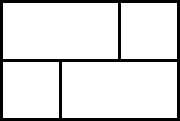
\includegraphics[scale=.5]{../Bwinf-Aufgabe1-KunstDerFuge/visualisierung/mauer-2.pdf}
\par\vspace{1em}
$n = 3$\\
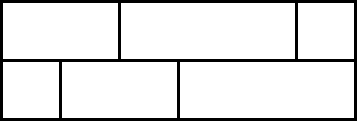
\includegraphics[scale=.5]{../Bwinf-Aufgabe1-KunstDerFuge/visualisierung/mauer-3.pdf}
\par\vspace{1em}
$n = 4$\\
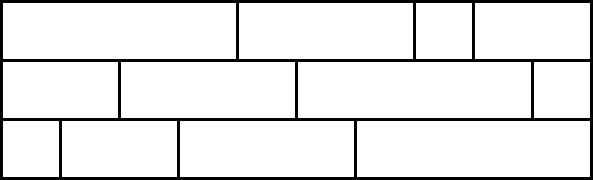
\includegraphics[scale=.5]{../Bwinf-Aufgabe1-KunstDerFuge/visualisierung/mauer-4.pdf}
\par\vspace{1em}
$n = 5$\\
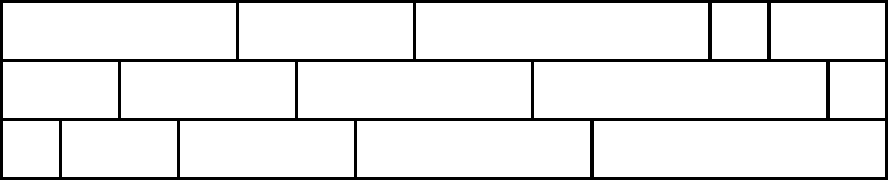
\includegraphics[scale=.5]{../Bwinf-Aufgabe1-KunstDerFuge/visualisierung/mauer-5.pdf}
\par\vspace{1em}
$n = 6$\\
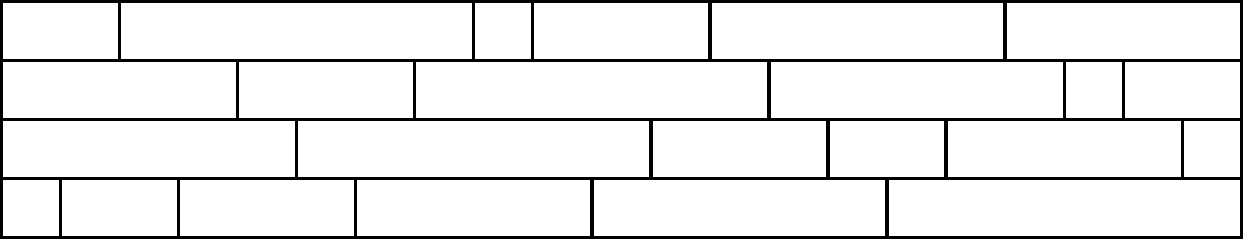
\includegraphics[scale=.5]{../Bwinf-Aufgabe1-KunstDerFuge/visualisierung/mauer-6.pdf}
\par\vspace{1em}
\newpage
$n = 7$\\
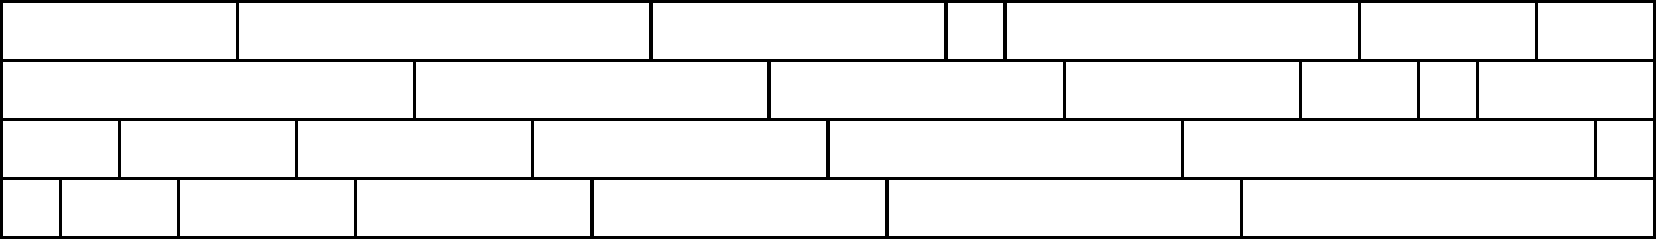
\includegraphics[width=\textwidth]{../Bwinf-Aufgabe1-KunstDerFuge/visualisierung/mauer-7.pdf}
\par\vspace{1em}
$n = 8$\\
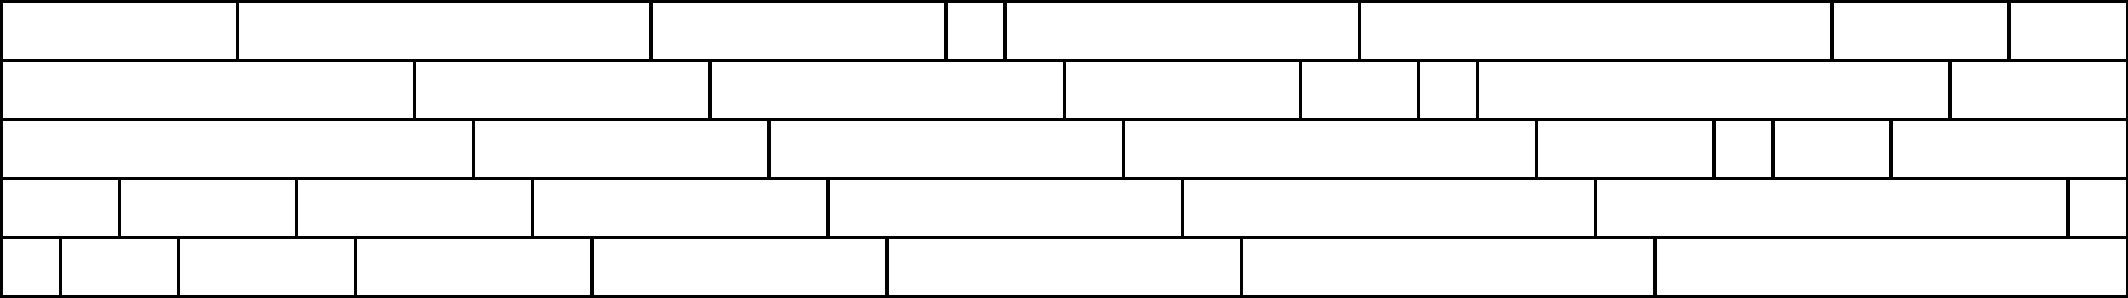
\includegraphics[width=\textwidth]{../Bwinf-Aufgabe1-KunstDerFuge/visualisierung/mauer-8.pdf}
$n = 9$\\
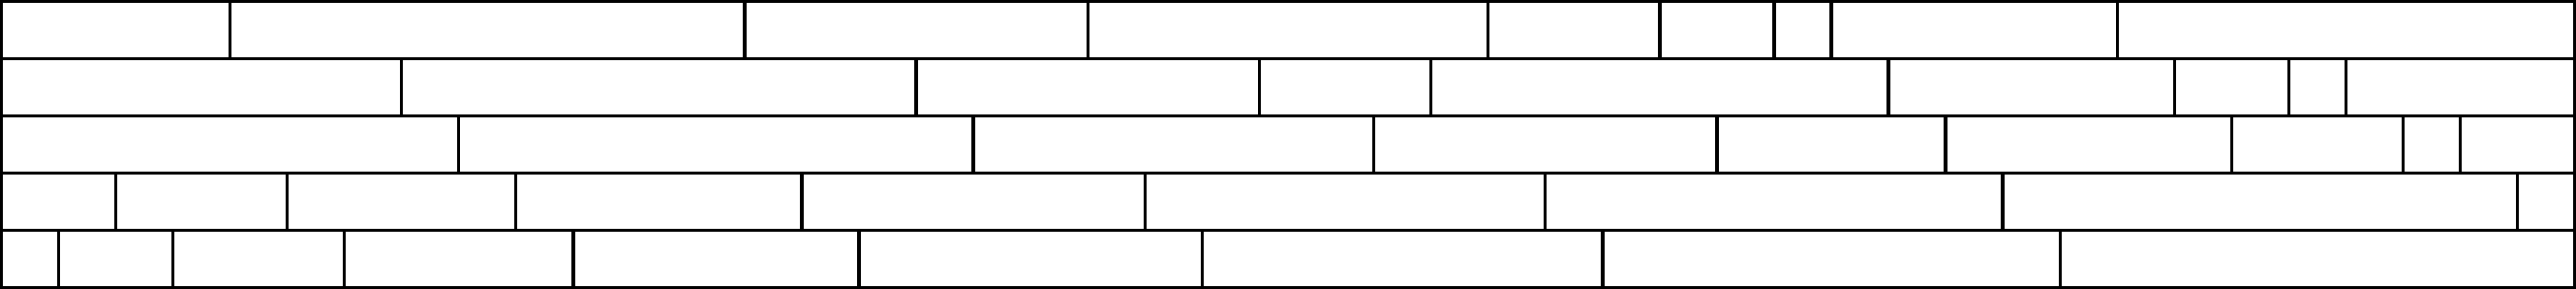
\includegraphics[width=\textwidth]{../Bwinf-Aufgabe1-KunstDerFuge/visualisierung/mauer-9.pdf}
\par\vspace{1em}
$n = 10$\\
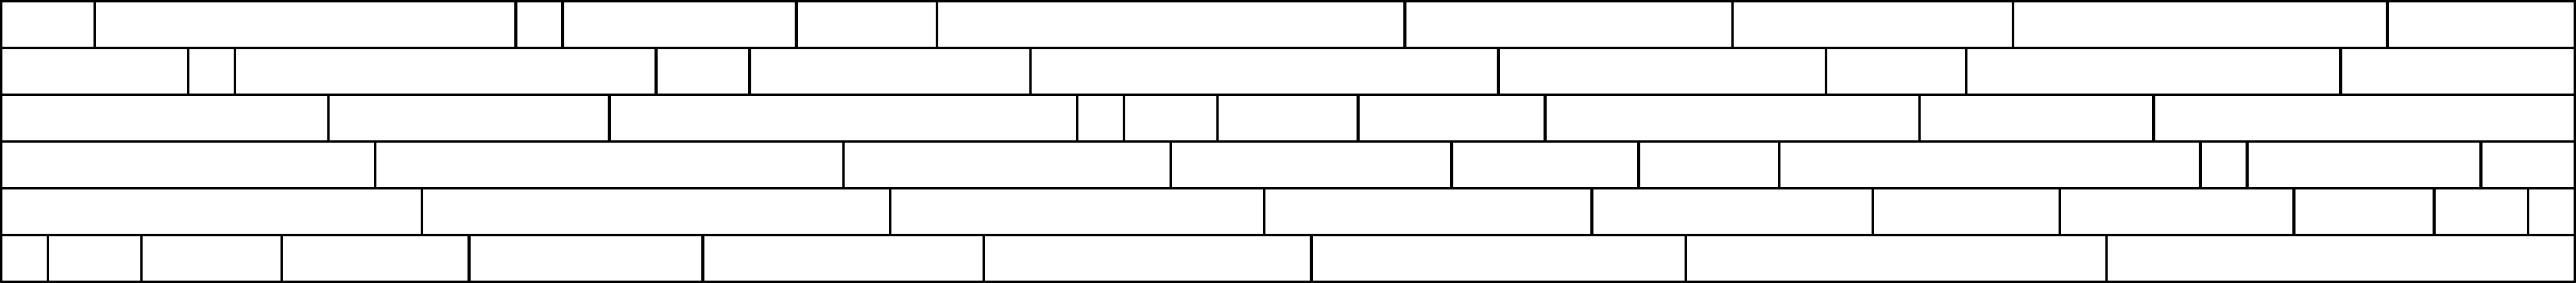
\includegraphics[width=\textwidth]{../Bwinf-Aufgabe1-KunstDerFuge/visualisierung/mauer-10.pdf}
\par\vspace{1em}
$n = 11$\\
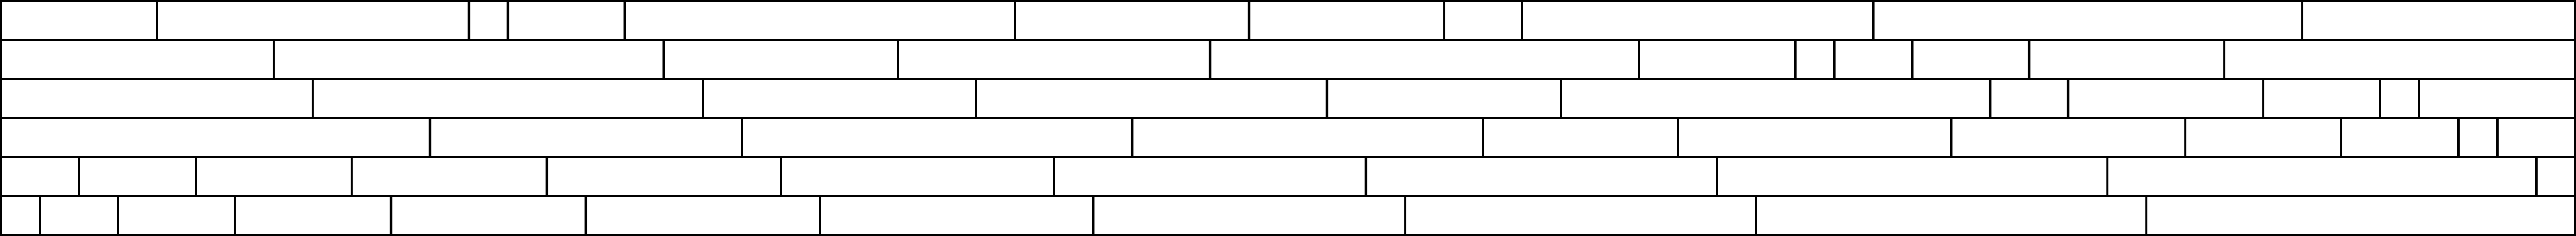
\includegraphics[width=\textwidth]{../Bwinf-Aufgabe1-KunstDerFuge/visualisierung/mauer-11.pdf}
\par\vspace{1em}
$n = 12$\\
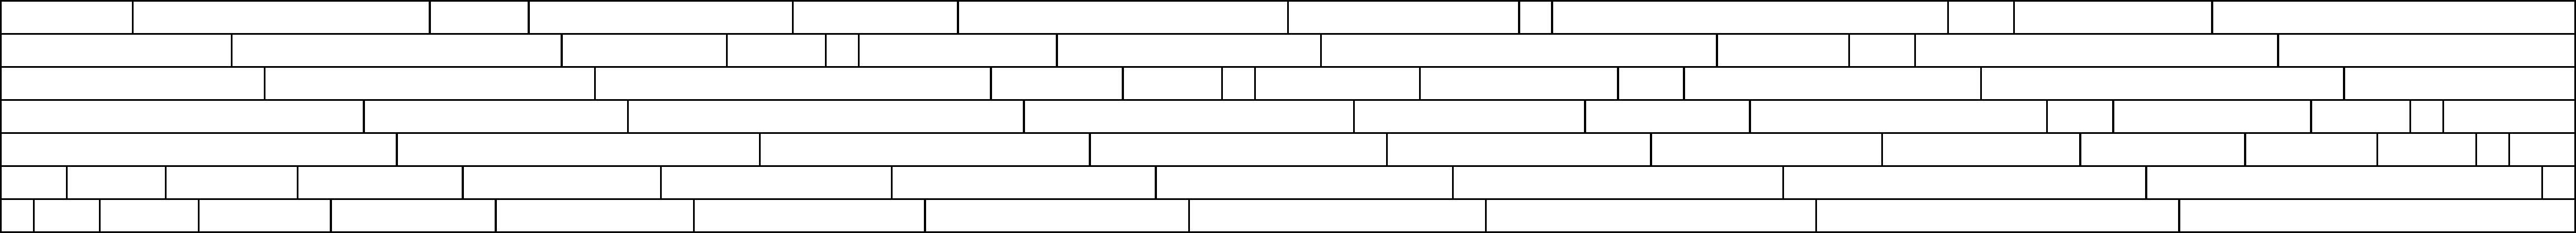
\includegraphics[width=\textwidth]{../Bwinf-Aufgabe1-KunstDerFuge/visualisierung/mauer-12.pdf}
\par\vspace{1em}
$n = 13$\\
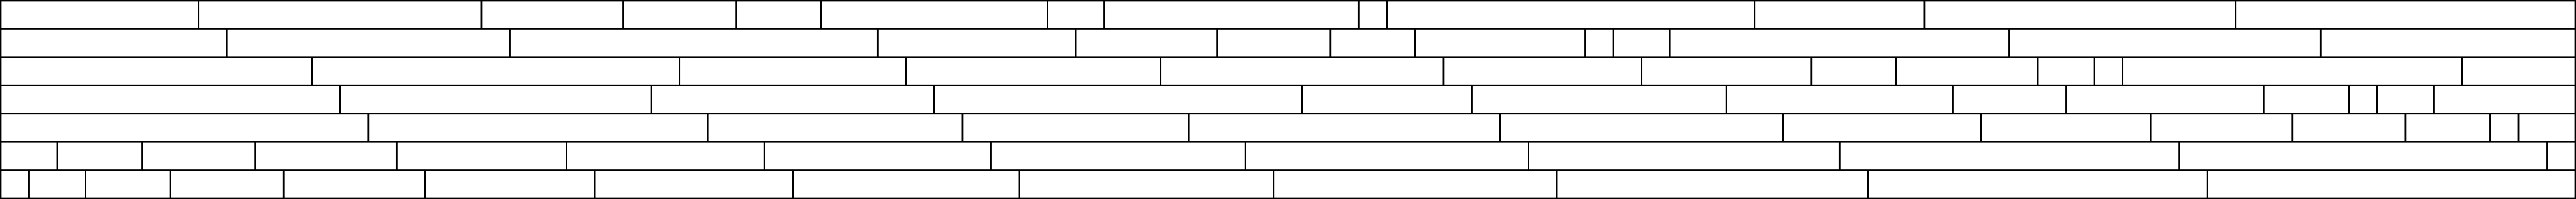
\includegraphics[width=\textwidth]{../Bwinf-Aufgabe1-KunstDerFuge/visualisierung/mauer-13.pdf}
\par\vspace{1em}
$n = 14$\\
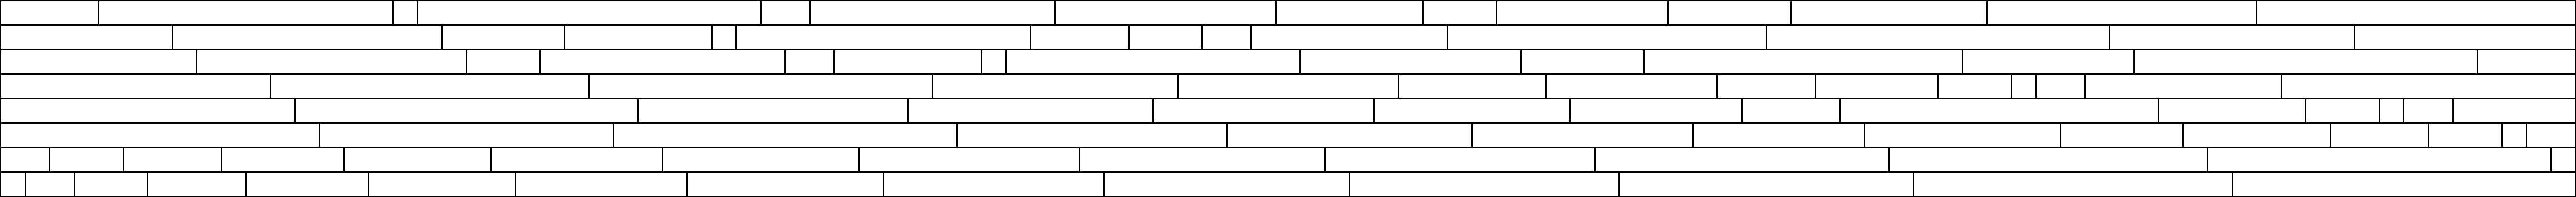
\includegraphics[width=\textwidth]{../Bwinf-Aufgabe1-KunstDerFuge/visualisierung/mauer-14.pdf}
\end{center}

 \section{Quellcode}
 \renewcommand{\listingscaption}{Quellcode}
 
 \begin{longlisting}
 \javafile{../Bwinf-Aufgabe1-KunstDerFuge/src/de/lukasrost/bwinf2017/r2_1/Main.java}
 \caption{\texttt{Main.java}}
 \end{longlisting}
 
 \end{document}